\documentclass[a4paper, 12pt]{article}

\usepackage{graphicx}
\usepackage{indentfirst}
\usepackage{enumitem}
\usepackage{geometry}
\geometry{left=3cm, right=3cm, top=2cm, bottom=2cm}
\usepackage{listings}
\usepackage{xcolor}
\definecolor{commentgreen}{RGB}{2,112,10}
\definecolor{eminence}{RGB}{108,48,130}
\definecolor{weborange}{RGB}{255,165,0}
\definecolor{frenchplum}{RGB}{129,20,83}
\usepackage[colorlinks,linkcolor=blue]{hyperref}
\setlength{\parindent}{2em}
\setlength{\parskip}{0.5em}
\usepackage{xltxtra}
\usepackage[ruled,linesnumbered]{algorithm2e}
\usepackage{amsmath}
\usepackage{amssymb}
\usepackage{textcomp}
\usepackage{tikz}

\newcommand{\HRule}{\rule{\linewidth}{0.5mm}}

\begin{document}

\lstset {
    language=C,
   frame=tb,
    tabsize=4,
    showstringspaces=false,
    numbers=left,
    %upquote=true,
    commentstyle=\color{commentgreen},
    keywordstyle=\color{eminence},
    stringstyle=\color{red},
    basicstyle=\small\ttfamily, % basic font setting
    emph={int,char,double,float,unsigned,void,bool},
    emphstyle={\color{blue}},
    escapechar=\&,
    % keyword highlighting
    classoffset=1, % starting new class
    otherkeywords={>,<,;,-,!,=,~},
    morekeywords={>,<,;,-,!,=,~},
    keywordstyle=\color{weborange},
    classoffset=0,
}

\begin{titlepage}
    \begin{center}
      % logo
      
\includegraphics[width=0.75\textwidth]{figure/polyulogo.png}~\\[1cm]
  
      \textsc{\large COMP2432 Operating Systems \\ Spring 2024}\\[3cm]
  
  
      \HRule \\[0.4cm]
      {\large \bfseries A Steel-Making Production Line Scheduler (PLS) \\ Project Report \\[0.4cm]}
      \HRule \\[4cm]
        \textbf{\large Group 07 \\}
      Wang Ruijie, Zhu Jin Shun, Zeng Tianyi, Liu Yuyang and Li Haoxuan \\[8cm]
  
      \vfill
  
      {\today}
  
    \end{center}
\end{titlepage}

\tableofcontents
\newpage

\section{Abstract}

Scheduling is a fundamental concept of significance for the multiprogramming operating systems.
By optimizing the throughput and resource cost, a system can achieve higher efficiency and better performance while handling multiple processes.
On the basis of the operating system scheduling algorithms that have been commonly researched and adapted, we are concentrated on modifying and applying the principles of the
algorithms to a real-world production scheduling scenario, and its implementation in the C programming language to construct schedulers with appropriate scheduling algorithms 
to model and optimize the problem. 

This report commences with our identifying of the concepts behind the scheduling algorithms, then followed by the adaptations of our modified scheduling algorithms to the production scheduling scenario with our deep investigation.
Afterwards, we display various technical details during the design and the implementation of the system, including our object-oriented design, system structure, process management, and inter-process communication.
With the given testing cases, the report then proceeds to the analysis of performance and the discussion of the results, and finally concludes the project.

\section{Introduction}

The objective of the system we have devised is to resolve a significant production scheduling issue confronting a medium-sized steel-making plant. 
The company has three manufacturing facilities with varying production capacities, each engaged in the production of distinct steel products. 
However, due to suboptimal production allocation and inefficient scheduling, the company was experiencing challenges such as order delays and reduced profitability. 
Consequently, our objective is to develop an integrated scheduling application that could effectively address these issues.

The impetus behind this project is to apply the principles of process scheduling learned in the field of operating systems to a real-world scenario. 
The objective is to create a scheduling application that would provide manufacturers with an efficient and optimized solution to plan and manage their production schedules. 
The ultimate goal is to maximize the utilization of the three factories to ensure optimal allocation of resources and timely fulfillment of orders.

The program's significance lies in its ability to enhance both short-term profitability and the company's long-term reputation and customer satisfaction. 
By implementing intelligent scheduling algorithms and analyzing different production scenarios, we can determine the most efficient utilization of the three plants. 
This will increase operational efficiency, reduce production bottlenecks and improve profitability. 


\section{Scope and Concepts}

What the project mainly focuses on are the scheduling algorithms that has been used by the modern operating systems, and also the imitative application of those scheduling algorithm to a real-world scenario in the production scheduling. However,
since the object we investigated, the steel-making production line, does not work under an ideal assumption, that is, there are more constraints and requirements compared with the operating systems, we have to find out the distinctions of the properties of the algorithms between the real-world scenario and the computer systems,
and eventually make necessary modifications.

In the context of operating systems, scheduling is regarded as the action of assigning resources to tasks.
The scheduling algorithms are used to allocate the CPU time to different processes, and the goal is to maximize the throughput, minimize the turnaround time, and optimize the resource utilization.
At the same time, other factors such as response time and fairness are also considered based on different kinds of tasks to be allocated to the CPU, e.g., interactive tasks and batch tasks, for which the judgement of the efficiency of the algorithms may differs greatly.
Another concept of importance is that, the scheduling algorithms can be classified into two categories, preemptive and non-preemptive, to determine whether the CPU can be taken away from the current process before it finishes its execution.
Apart from the results of the algorithms, the complexity of the schedulers themselves can also influence their performance.
Exactly because of the above considerations, programmers have already developed a variety of scheduling algorithms, such as First-Come-First-Served (FCFS), Shortest-Job-First (SJF), Round-Robin (RR), Priority Scheduling (PR), and Multilevel Queue Scheduling, to meet all kinds of requirements.
By referring to the project description, we can see the following differences in the given situation: 

\begin{enumerate}
    \item A new concept of due date is put forward which indicates the deadline of the orders, and we have to find out the best allocation before such a moment, while it is not emphasized in CPU scheduling; 
    \item We are with the ability to refuse some of the orders, where more acceptance of the orders does not indicates a higher utilization or efficiency;
    \item There are three production lines being allocated concurrently in an asynchronous way, which means that the orders can be processed in parallel, while the CPU scheduling is a serial and synchronous process;
    \item The orders are considered to be without the concept of arrival time, i.e., they are all available at the beginning of the period, which is different from the CPU scheduling where the processes are generated dynamically;
    \item The cost of context switching is much more notable, as a factory can only process one order at a day.
\end{enumerate}

We also refer to the ideas from operations research to model the given scenario and try to optimize the outcomes. For problems whose requirements and objective are represented by linear relations,
linear programming, especially, simplex methods, are introduced. For each of the orders, the number of days allocated to each factory denoted by non-negative integers $x, y$ and $z$ respectively, can be the variables to be optimized.
We are expected find a vector $v = (x, y, z)$ such that maximizes the efficiency or utilization, or minimizes the cost, under the constraints that the sum of the days allocated to each order is less than the number of days available, and the sum of the days allocated to each factory is equal to the total number of days.
With such a model, we can rethink the scenario and the problem of scheduling in a mathematical and algorithmic way.

\section{Scheduling Algorithms Adapted}

\subsection{Smallest Remaining First (SRF)}

In the context of the operating systems the Smallest Remaining First (SRF) algorithm is a preemptive scheduling algorithm that selects the task with the smallest remaining processing time to execute next. 
However, because the order of task arrival is not considered, and the order with the smallest quantity will not change once it is found and before it has been decided the place of allocation,
this algorithm can be seen as a non-preemptive one, even though if the orders do not come at the same time, the algorithm will still work with preemption.

We define the criterion of determine the smallest remaining as the quantity of an order. For each day of the given period, the algorithm iteratively goes through all orders and selects the one with the smallest quantity to process in each iteration.
After that, it will place the order into one or more factories of the day based on our special placement strategy, to reach a greedy optimization that the capacity waste of the day is minimized. The algorithm 
is demonstrated in the following pseudo code:

\begin{algorithm}[H]
    \For{each day of the period} {
        \If{all orders have been allocated} {
            break\;
        }
        \If{all factories are occupied} {
            continue\;
        }
        smallest quantity = INT\textunderscore MAX\;
        \For{each order of all the orders} {
            \If{quantity of the order < smallest quantity \\ AND the order has not been refused \\ AND the order has not been completed} {
                smallest quantity = quantity of the order\;
                order with smallest quantity = order\;
            }
        }
        allocate the selected order to the available factories of the day with the greedy strategy\;
    }
    \caption{Smallest Remaining First (SRF) Algorithm}
\end{algorithm}

Especially, the greedy strategy of allocating the selected order with smallest quantity to the available factories of that day is designed as follows. 
We can see that for each turn, the strategy will try to allocate the order to the factory with the smallest capacity that can just cover the quantity of the order, 
or the maximum factory capacity that is not enough to complete the order, which ensures that the order can be finished as soon as possible and the waste capacity of the factories is minimized.
From the perspective of each allocation, the strategy is optimal in maximize the utilization of a factory in that day for a given order. 
However, in the global view, it is hard to reach the highest utilization of all factories for all orders during the whole period.

\begin{algorithm}[H]
    $x$ = the capacity of factory X\;
    $y$ = the capacity of factory Y\;
    $z$ = the capacity of factory Z\;
    $q$ = the quantity of the selected order\;
    \If{all factories are available} {
        \If{$q \leq x$} {
            allocate the order to factory X\;
        } \ElseIf {$q \leq y$} {
            allocate the order to factory Y\;
        } \ElseIf {$q \leq z$} {
            allocate the order to factory Z\;
        } \ElseIf {$q \leq x + y$} {
            allocate the order to factory X and Y\;
        } \ElseIf {$q \leq x + z$} {
            allocate the order to factory X and Z\;
        } \ElseIf {$q \leq y + z$} {
            allocate the order to factory Y and Z\;
        } \Else {
            allocate the order to all factories\;
        }
    }
    \If{factory X is occupied} {
        ...
    }
    \If{factory Y is occupied} {
        ...
    }
    \If{factory Z is occupied} {
        ...
    }
    \If{factory X and Y are occupied} {
        ...
    }
    \If{factory X and Z are occupied} {
        ...
    }
    \If{factory Y and Z are occupied} {
        ...
    }
    Update the availability of the factories\;
    Update the remaining quantity and the completion of the order\;
    \caption{Greedy Strategy of Order Allocation of a Day}
\end{algorithm}

\subsection{Earliest Due Date Priority (PR)}

Instead of using the category of the product, we believe that it might be more reasonable to use the due date of the order as the priority. The closer
the due date is, the higher the priority is. Similarly, since the order is statistically stored, the algorithm will not perform any preemption. 
The algorithm can be demonstrated in the following pseudo code:

\begin{algorithm}[H]
    \For{each day of the period} {
        \If{all orders have been allocated} {
            break\;
        }
        \If{all factories are occupied} {
            continue\;
        }
        earliest due date = INT\textunderscore MAX\;
        \For{each order of all the orders} {
            \If{due date of the order < earliest due date \\ AND the order has not been refused \\ AND the order has not been completed} {
                earliest due date = due date of the order\;
                order with earliest due date = order\;
            }
        }
        allocate the selected order to the available factories of the day\;
    }
    \caption{Earliest Due Date Priority (PR) Algorithm}
\end{algorithm}

The greedy strategy of order allocation of a day is still utilized in the Earliest Due Date Priority algorithm to achieve the local optimization of the factories' utilization.

\subsection{Smallest Global Waste (SGW)}

In the Smallest Remaining First (SRF) and the Earliest Due Date Priority (PR) algorithms, the greedy allocation of an order is limited, since they requires the orders should be completed as soon as possible if possible.
If not, the order will be rejected. Moreover, without preemption, the two aforementioned algorithms can be viewed as online algorithms 
operating under the constraint of incomplete information during planning. They are unable to transcend the limitations of the information accessible to them, basing their decisions and selections solely on the available data. 
That is, during each processing instance, they are only privy to the information pertaining to the various factories for a particular day.

Acknowledging the limitations of the SRF and PR algorithms, we introduce an improvement of the algorithms,
the Smallest Global Waste (SGW) algorithm, which is designed to optimize the overall waste across all factories and days.
This algorithm is preemptive for a given order. In each iteration, the algorithm traverses the linked list of the orders from the head to the tail,
and finds out the best division of the quantity of the order to different factories and different dates. 

For example, if an order of the quantity 1000 is selected to allocate in the SRF or PR algorithm in the condition that all factories are available,
the order will be allocated to the factories X, Y and Z. The waste of the capacity is $300+400+500-1000 = 200$. 
With reference to the SGW algorithm, the order will be allocated to the factory Z twice in two days, and no waste is generated.

Set $x_i, y_i, z_i$ as the capacities of the factories X, Y and Z respectively for the iteration $i$, and $q_i$ as the quantity of the selected order. We can translate the idea of the SGW algorithm into the following linear programming problem:

\begin{equation*}
    \begin{array}{ll@{}ll}
    \text{minimize}  & \displaystyle 300x_i+400y_i+500z_i - q_i,      &\\
    \text{subject to}& \displaystyle 300x_i+400y_i+500z_i \geq q_i,  \qquad  & i = 1 ,\dots, n\\
                     &  \displaystyle \sum_{i=1}^{n}x_i = \sum_{i=1}^{n}y_i = \sum_{i=1}^{n}z_i  = n,          & x_i, y_i, z_i \in \mathbb{N} \\
    \end{array}
\end{equation*}

Thanks to the GLPK (GNU Linear Programming Kit) package, we can compute the desired results. Therefore, the SGW algorithm is designed as follows:

\begin{algorithm}
    n = the number of days of the period\;
    remaining days of factory x = n\;
    remaining days of factory y = n\;
    remaining days of factory z = n\;
    \For {each order of the all} {
        \If {the optimal x', y', z' can be found considering the remaining days} {
            x = x - x'\;
            y = y - y'\;
            z = z - z'\;
            occupy x', y', z' days of the factories x, y, z respectively\;
            modify the acceptance and completion states of the order\;
        }
        \Else {
            refuse the order\;
        }
    }
    \caption{Smallest Global Waste (SGW) Algorithm}
\end{algorithm}

One disadvantage of the SGW algorithm is that it is computationally expensive, and the complexity of the algorithm is $\mathcal{O}(n^2)$, where $n$ is the number of orders.
Meanwhile, it is still a greedy algorithm for each order, i.e., the orders are processed in the first-come-first served way.

\section{Design and Implementation}

We will displays various technical details in the design and implementation of the program with the C programming language and Unix/Linux system calls.

\subsection{Object-Oriented Design}

For the convenience of the manipulation of the data of the objects and the better organization of the program, we adapt the object-oriented programming paradigm
to model and construct the classes of \texttt{order}, \texttt{factory} and \texttt{day} in separated header files \texttt{order.h}, \texttt{factory.h} and \texttt{day.h} respectively.
Their functions are realized in the corresponding source files \texttt{order.c}, \texttt{factory.c} and \texttt{day.c} respectively. For each of the classes, we prepare
the creator, getter, and setter functions to initialize the objects, access the attributes, and modify the attributes respectively. The classes are defined as follows:

\begin{itemize}
    \item \texttt{order} class includes the basic attributes of an order, such as the order number, the quantity, and the due date. To realize the dynamic storing of the orders with a linked list,
    a \texttt{next} pointer pointing to the next order is added. Meanwhile, two supplementary boolean attributes \texttt{is\textunderscore completed} and \texttt{is\textunderscore accepted} are added as well to indicate the 
    alteration of the order status during the processing. 
    \item \texttt{factory} class includes the basic attributes of the factory name, the capacity, the order that the factory is processing in that day, and the availability of the factory of that day. Please note that 
    \texttt{factory} objects are defined for each day, and the factories are allocated in an asynchronous way. Three different creators for the three factories are defined to initialize the factories with different capacities.
    \item \texttt{day} class can be considered as a set of all information about the three factories of a day. For each day of the given period, a \texttt{day} object is created to store the factories of that day. Through a \texttt{day} object,
    all information are accessible, including the factories, the orders processed on that day, and the allocation of the orders. When a \texttt{day} object is created, the factories are also initialized respectively. Similar 
    to the \texttt{order} class, a \texttt{next} pointer is added to realize the dynamic storing of the days with a linked list.
\end{itemize}

\subsection{Data Structures}

With the help of the object-oriented design, it is easy to realize the dynamic storing of the orders and the days with the linked list data structure, making the program more flexible and scalable 
when a huge amount of data is imported. In the main function, a constant pointer \texttt{order\textunderscore head} is set to point to the head of the linked list of the orders
throughout the program. The contents of the orders, stored in the linked list pointed by the \texttt{day\textunderscore head}, will not be modified, and it can be copied to another linked list for further processing.
While the \texttt{order\textunderscore head} pointing to the contents of factories and orders allocation of the period, it will be initialized only when a \texttt{runPLS} command is passed, as in the process of scheduling, some of the contents such as the status of the orders and the factories can be updated accordingly.
To get any required information, it suffices just to traverse the linked list of the orders and the days, which has to a good time complexity of $\mathcal{O}(n)$.

\subsection{System Structure and Process Management}

Besides the header files and their corresponding source files that implements the object-oriented design, the system is generally deployed within \texttt{PLS\textunderscore G07.c}, where the main function is located.
Functions that are repeatedly called are independent of the main function, including the greedy strategy of allocating the orders to the factories and other specialized helper functions. 

Collectively, the program is divided into four modules: the input module, the scheduling module, the output module, and the analysis module, and each of them owns a process. 
At the beginning of the execution, the main process (taking the role of the input module) will fork once, and then the child process (taking the role of the scheduling module) will fork once again (get the grandson process which takes the role of the output module).
Therefore, there will be three processes running throughout the execution. 
As for the analysis module, it will not be created until the command \texttt{runPLS} is passed. In that case, the scheduling module will fork once again to create the analysis module that is responsible for generating the analysis report.
After the part of scheduling is completed and outputted, the analysis module will immediately exit and collected by the scheduling module.

Each module except the analysis module is running in a loop until receiving the message to exit, and the logics of each module are basically independent of each other. 
The only counterexample is the communication between the scheduling module and the output module, which will be explained in the next section.

From the perspective of the functionality, the input module only takes the responsibility of reading and passing the commands,
while the scheduling module is responsible for parsing, scheduling, and passing the useful information to the output module.
It also takes the role of generating the raw input file \texttt{input\textunderscore commands.txt}.
Both the output module and the analysis module are essentially take the same role for generating output, but the analysis module is used and discarded with short lifespan,
and access the information by \texttt{fork()} to inherit the memory space of the scheduling module.

\begin{figure}[htbp]
    \centering
    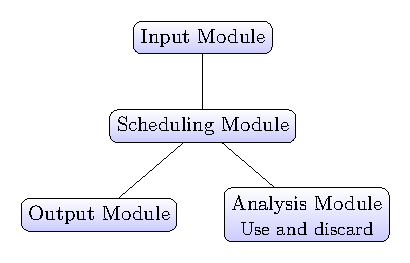
\includegraphics[width=0.6\textwidth]{figure/tikz_pic1.pdf}
    \caption{System Structure}
\end{figure}

\subsection{Inter-Process Communication}

The inter-process communication is realized by the Unix/Linux system calls \texttt{pipe()} and \texttt{fork()}. Before each \texttt{fork()}, two uni-directional unnamed pipes will be created to establish the bi-directional communication between the parent process and the child process.
The pipes are set to be blocking mode by default to ensure the synchronization of the processes.

With reference to the system structure, the line communication topology is adopted, for most of the messages are intended to be 
handled by the scheduling module. The line communication topology is more efficient other topologies for our centralized structure.
The analysis module is not on the line since it is able to inherit the accessability to the data of the scheduling module by \texttt{fork()}.

An important detail of our inter-process communication mechanism is the method of ensuring that the receiver module is able to
read the desired message and recognize it. The time difference between the sender module's writing and the receiver module's reading 
leads to possible blocking of the both modules. To avoid this trouble, the receiver module has to read from the pipe in a loop until
the message read is different from the previous one, which is stored in the previous buffer. By doing so, the receiver can always read a new message with 
unavoidable delay, and proceeds to compare the message with the predefined ones to determine the next step to take.
The receiver module might send back a signal message to indicate it is ready to continue. To display this, we provide an example below:

\begin{lstlisting}
// Sender module (scheduling module)

/**
* Tell the output module to print the report
*/
write(scheduling_to_output[1], "prrp", 4);

/**
* If the response is "OK2", send the file name to the output module
*/
strcpy(previous_buffer, buffer);
while(strcmp(buffer, previous_buffer) == 0) {
    read(output_to_scheduling[0], buffer, MAX_BUFFER_SIZE);
    buffer[3] = '\0';
}
if (strcmp(buffer, "OK2") == 0) {
    write(scheduling_to_output[1], tokens[5], strlen(tokens[5]) + 1);
}
\end{lstlisting}

\begin{lstlisting}
// Receiver module (output module)

/**
* If the contents of the buffer are the same as the previous buffer, 
* there is no new message
* Keep reading from the scheduling module until a new message is received
*/
char previous_buffer[MAX_BUFFER_SIZE];
strcpy(previous_buffer, buffer);
while(strcmp(buffer, previous_buffer) == 0) {
    read(scheduling_to_output[0], buffer, MAX_BUFFER_SIZE);
}
buffer[4] = '\0';

if (strcmp(buffer, "prrp") == 0) {
    write(output_to_scheduling[1], "OK2", 3);
    
    strcpy(previous_buffer, buffer);
    while(strcmp(buffer, previous_buffer) == 0) {
        read(scheduling_to_output[0], buffer, MAX_BUFFER_SIZE);
    }
    printf("saved to file %s\n", buffer);
    // continue...
}
\end{lstlisting}

The code above demonstrates the process of scheduling module asking the output module to print the report and sending the file name to the output module.
The output module will keep reading from the scheduling module until a new message is received, and then print the file name to the screen.
Meanwhile, the output module will send back the signal message ``OK2" to the scheduling module 
if the signal message ``prrp'' is well-received to indicate that it is ready to receive the file name.

There are various similar cases in the program, especially during the process of massive message exchange, e.g.,
the passing of scheduling result line by line to the output module.
We are inspired by the idea of the ACK mechanism from the TCP connection protocol and the reliable data transfer (rdt) mechanism.
Since the pipe message queue is large enough, we can assume the inter-process communication via pipes as a reliable data transfer over a reliable channel (rdt1.0).

\subsection{Input and Output Handling}

The input module utilizes an infinite loop to read the user input from the standard input stream. The input module
only detects whether the input is \texttt{exitPLS} or not to decide whether to start to wait for the child processes. 

Whatever the input is, the input module will send a message via the pipe to the scheduling module in the form of a string.
Two important functions, \texttt{char** get\_tokens\_from\_input(char *input)} and 
\texttt{char** get\_store\_tokens\_from\\ \_input(char *input)},
for parsing the input string are defined to split the string with spaces and return the tokens by calling \texttt{strtok} function, while the latter function will store the received string to the \texttt{input\_commands.txt}.
By comparing the indicated position of the tokens with the predefined commands, the scheduling module can determine the next step to take.

Both the output module and the analysis module are responsible for generating and export the output to the specified output files. 
Once \texttt{runPLS} is passed, the analysis module will open the file \texttt{analysis\_report.txt} and write the analysis report to the file.
For the output module, only when \texttt{runPLS} is followed by \texttt{printREPORT}, the output module will open the file with 
the given file name and write the output to the file.

The function \texttt{void clear\_file(char *file\_name)} is called at the beginning of the main function to clear the contents of \texttt{input\_command.txt} and \texttt{analysis\_\\report.txt}, by opening the file with ``w'' method, which 
will create a new file if the file does not exist and clear the content of the file if the file exists. When \texttt{printREPORT} is passed, the output file will also be cleared before writing the output to the file.
After that, all the output functions will append the output to the file with the ``a'' method. Within each execution, the contents will not be cleared again.

\section{Testing}

An effective way to test the correctness is to use the input we prepare in the system, that is, an order with large quantity. 
We expect that no factory can process the order, and the order will be refused.
If this is the case, the correctness of the program can be guaranteed.

User input:
\begin{lstlisting}
addPERIOD 2024-04-01 2024-04-10
addORDER P001 2024-04-02 8000 PA
runPLS SRF | printREPORT > output_1_1.txt
runPLS PR | printREPORT > output_1_2.txt
runPLS SGW | printREPORT > output_1_3.txt
\end{lstlisting}

Output:
\begin{lstlisting}
//output_1_1.txt
----------------
2024-04-01 x N/A N/A N/A N/A
----------------
2024-04-01 y N/A N/A N/A N/A
----------------
2024-04-01 z N/A N/A N/A N/A
----------------
2024-04-02 x N/A N/A N/A N/A
----------------
2024-04-02 y N/A N/A N/A N/A
----------------
2024-04-02 z N/A N/A N/A N/A
----------------
2024-04-03 x N/A N/A N/A N/A
----------------
2024-04-03 y N/A N/A N/A N/A
----------------
2024-04-03 z N/A N/A N/A N/A
----------------
2024-04-04 x N/A N/A N/A N/A
----------------
2024-04-04 y N/A N/A N/A N/A
----------------
2024-04-04 z N/A N/A N/A N/A
----------------
2024-04-05 x N/A N/A N/A N/A
----------------
2024-04-05 y N/A N/A N/A N/A
----------------
2024-04-05 z N/A N/A N/A N/A
\end{lstlisting}

\begin{lstlisting}
//output_1_2.txt
----------------
2024-04-01 x N/A N/A N/A N/A
----------------
2024-04-01 y N/A N/A N/A N/A
----------------
2024-04-01 z N/A N/A N/A N/A
----------------
2024-04-02 x N/A N/A N/A N/A
----------------
2024-04-02 y N/A N/A N/A N/A
----------------
2024-04-02 z N/A N/A N/A N/A
----------------
2024-04-03 x N/A N/A N/A N/A
----------------
2024-04-03 y N/A N/A N/A N/A
----------------
2024-04-03 z N/A N/A N/A N/A
----------------
2024-04-04 x N/A N/A N/A N/A
----------------
2024-04-04 y N/A N/A N/A N/A
----------------
2024-04-04 z N/A N/A N/A N/A
----------------
2024-04-05 x N/A N/A N/A N/A
----------------
2024-04-05 y N/A N/A N/A N/A
----------------
2024-04-05 z N/A N/A N/A N/A
\end{lstlisting}

\begin{lstlisting}
//output_1_3.txt
----------------
2024-04-01 x N/A N/A N/A N/A
----------------
2024-04-01 y N/A N/A N/A N/A
----------------
2024-04-01 z N/A N/A N/A N/A
----------------
2024-04-02 x N/A N/A N/A N/A
----------------
2024-04-02 y N/A N/A N/A N/A
----------------
2024-04-02 z N/A N/A N/A N/A
----------------
2024-04-03 x N/A N/A N/A N/A
----------------
2024-04-03 y N/A N/A N/A N/A
----------------
2024-04-03 z N/A N/A N/A N/A
----------------
2024-04-04 x N/A N/A N/A N/A
----------------
2024-04-04 y N/A N/A N/A N/A
----------------
2024-04-04 z N/A N/A N/A N/A
----------------
2024-04-05 x N/A N/A N/A N/A
----------------
2024-04-05 y N/A N/A N/A N/A
----------------
2024-04-05 z N/A N/A N/A N/A
\end{lstlisting}

\section{Performance Analysis}

\begin{lstlisting}
***PLS Schedule Analysis Report***
Algorithm used: SRF
0 orders ACCEPTED. Details are as follows:
ORDER NUMBER     START           END         DAYS        QUANTITY        PLANT
===========================================================================================
- END -



==========================================================================================================


There are 1 Orders REJECTED.    Details are as follows:

ORDER NUMBER    PRODUCT NAME    DUE DATE    QUANTITY

==========================================================================================================

P001         pa          2024-04-02          5600
- END -


===========================================================================================================


***PERFORMANCE

PLANT_X:
Number of days in use: 0 days
Number of products produced: 0 (in total)
Utilization of the plant: -nan %
PLANT_Y:
Number of days in use: 0 days
Number of products produced: 0 (in total)
Utilization of the plant: -nan %
PLANT_Z:
Number of days in use: 0 days
Number of products produced: 0 (in total)
Utilization of the plant: -nan %

Overall utilization: -nan %
- END -
***PLS Schedule Analysis Report***
Algorithm used: PR
0 orders ACCEPTED. Details are as follows:
ORDER NUMBER     START           END         DAYS        QUANTITY        PLANT
===========================================================================================
- END -



==========================================================================================================


There are 1 Orders REJECTED.    Details are as follows:

ORDER NUMBER    PRODUCT NAME    DUE DATE    QUANTITY

==========================================================================================================

P001         pa          2024-04-02          5600
- END -


===========================================================================================================


***PERFORMANCE

PLANT_X:
Number of days in use: 0 days
Number of products produced: 0 (in total)
Utilization of the plant: -nan %
PLANT_Y:
Number of days in use: 0 days
Number of products produced: 0 (in total)
Utilization of the plant: -nan %
PLANT_Z:
Number of days in use: 0 days
Number of products produced: 0 (in total)
Utilization of the plant: -nan %

Overall utilization: -nan %
- END -
***PLS Schedule Analysis Report***
Algorithm used: SGW
0 orders ACCEPTED. Details are as follows:
ORDER NUMBER     START           END         DAYS        QUANTITY        PLANT
===========================================================================================
- END -



==========================================================================================================


There are 1 Orders REJECTED.    Details are as follows:

ORDER NUMBER    PRODUCT NAME    DUE DATE    QUANTITY

==========================================================================================================

P001         pa          2024-04-02          5600
- END -


===========================================================================================================


***PERFORMANCE

PLANT_X:
Number of days in use: 0 days
Number of products produced: 0 (in total)
Utilization of the plant: -nan %
PLANT_Y:
Number of days in use: 0 days
Number of products produced: 0 (in total)
Utilization of the plant: -nan %
PLANT_Z:
Number of days in use: 0 days
Number of products produced: 0 (in total)
Utilization of the plant: -nan %

Overall utilization: -nan %
- END -
\end{lstlisting}

\section{Program Configuration and Execution}

Since the object-oriented programming paradigm is adapted in the program, the definitions of the classes of \texttt{order}, \texttt{factory} and \texttt{day} and their functions are given in three header files \texttt{order.h}, \texttt{factory.h} and \texttt{day.h} respectively. 
The implementation of the creator, getter,  and setter functions are written in three corresponding source files \texttt{order.c}, \texttt{factory.c} and \texttt{day.c} respectively. The main function is in \texttt{PLS\textunderscore G07.c}, where the header files are included and the functions are called insides.
Meanwhile, the header files and their source files are dependent on each other. 

Among those files, C standard libraries \texttt{stdio.h}, \texttt{string.h}, \texttt{stdlib.h}, \texttt{time.h}, \texttt{stdbool.h} and \texttt{limits.h} are also included for basic logics including but not limited to stream input and output handling, string manipulation, memory allocation, time manipulation, boolean values, and integer limits.
Two libraries related to the operating system, \texttt{unistd.h} and \texttt{sys/wait.h}, are also included for the system call \texttt{fork()}, \texttt{pipe()}, and \texttt{wait()} for creating child processes and inter-process communication.

An external library \texttt{glpk.h} is included for the simplex method to solve the linear programming problem. GLPK (GNU Linear Programming Kit) is a useful package for solving linear programming (LP), mixed integer programming (MIP), and other related problems. 
It is a set of routines written in ANSI C and organized in the form of a callable library. We introduces the simplex methods provided by GLPK to implement our third scheduling algorithm, the Smallest Global Waste (SGW) algorithm.

Accordingly, please ensure that the \texttt{gcc} compiler is set to support at least the ISO/IEC 9899:1999 C standard (C99). 
To include the GLPK library, please upload the \texttt{glpk-5.0.tar} file provided to the apollo machine. Afterwards, execute the following command to unarchive the file:
\textcolor{blue}{\texttt{tar -xf glpk-5.0.tar}}.


Then, go to the directory of the unarchived files and execute the following commands to install. Remember to 
replace my netID \texttt{22103808d} with your own path.
\begin{alignat}{1}
    &\textcolor{blue}{\texttt{cd ./glpk-5.0}} \nonumber \\
    &\textcolor{blue}{\texttt{./configure --prefix=/home/22103808d/myusr/local/lib/include}} \nonumber \\
    &\textcolor{blue}{\texttt{make}} \nonumber \\
    &\textcolor{blue}{\texttt{make install}} \nonumber
\end{alignat}

The procedure above may take a few minutes to complete. After that, 
use a text editor, e.g., \texttt{pico}, \texttt{nano}, or \texttt{vi}, to open the file \texttt{$\sim$/.bashrc}, and add the two lines to the file and save it:
\textcolor{blue}{\texttt{export C\_INCLUDE\_PATH=/home/22103808d/myusr/local/lib\\/include/include:\$C\_INCLUDE\_PATH}}, and
\textcolor{blue}{\texttt{export LD\_LIBRARY\_PATH=/home\\/22103808d/myusr/local/lib/include/lib:\$LD\_LIBRARY\_PATH}}. Remember 
to use your own path instead of mine as well.
Finally, execute the command \textcolor{blue}{\texttt{source $\sim$/.bashrc}} to make the changes take effect.

In order to run the program, please upload all C source files and header files (\texttt{order.h}, \texttt{factory.h}, \texttt{day.h}, \texttt{order.c}, \texttt{factory.c}, \texttt{day.c}, and \texttt{PLS\textunderscore G07.c})
to the same directory on \texttt{apollo}. Enter the directory, and input the command below to compile the program:
\textcolor{blue}{\texttt{gcc -o PLS\textunderscore G07 PLS\textunderscore G07.c order.c factory.c day.c \\-L/home/22103808d/myusr/local/lib/include/lib -lglpk}}.
Remember not to have a new line in between the command and use your own path. Finally, run the compiled executable file with the command
\textcolor{blue}{\texttt{./PLS\textunderscore G07}}.

After executing the program, you can see the prompt \texttt{Please enter: } on the screen, and you can input the commands according to the formats given in the project description.
Since for some of the commands the system will print the results to the screen, the prompt \texttt{Please enter: } may undergo a displacement, 
potentially appearing before the output content due to the lack of coordination among processes. If such a situation occurs, please continue to enter your commands.

We have done basic error handling for the input commands, e.g., if the due date of an order is later than the last date of the period, the due date will be set to the last date of the period, and 
if the due date is prior to the first date of the period, the order will be refused. However, if the elements of an input command are displaced or the command is not recognized, the program will not work properly.
We assume that \texttt{addPERIOD} is always the first command to be input, only \texttt{addORDER} commands are in the \texttt{.dat} file of \texttt{addBATCH}, and the \texttt{exitPLS} command is always executed before the user check the output files. If there is any error in the input commands, 
we strongly recommend you to restart the program for the correct execution.

\section{Results Discussion}

The given testing case can achieve the expected results, 
and the program is able to handle the input commands and generate the output and analysis files as required.

\section{Conclusion}

Generally speaking, our system for the steel-making production line scheduling problem are effective and efficient.
All requirements of the project description are met, and the program is stable enough to handle the tasks of input parsing, scheduling, output generation, and analysis exporting.
On the basis of these accomplishments, we also put forward innovative solutions throughout the project. 

\section{Miscellaneous}

This report of the project is written in \LaTeX, and it is built with the \TeX  Live Utility on macOS. The typesetting engine is \XeLaTeX. 
The report goes with a plain template rather than the IEEE template, and we make junior modifications to the required division of the report sections, but
all contents worthy of discussion are included. The source and work files of the report are stored in the \texttt{project\textunderscore report\textunderscore working\textunderscore directory} directory, and the source code is in the \texttt{source} directory for your reference.

The source code of the project has the unified style of indentation, naming conversion and commenting to make sure that the code is readable and maintainable.
We use the snake case for the naming of variables and functions, while the Doxygen style is adapted for the comments. 

We had worked on this project since 1 April, 2024, and we have spent 18 days on the project. The project is completed on 19 April, 2024.

\section{Innovation Highlights}

We believe that we have put forward original innovation solutions to the given problem with good performance:

\begin{enumerate}
    \item The improved SRF algorithm
    \item The special Earliest Due Date PR algorithm
    \item The SGW algorithm with the linear programming model
    \item The object-oriented design of the essential classes
    \item The inter-process communication mechanism for massive message exchanges
\end{enumerate}

The information about the innovations can be obtained from the corresponding sections for the detailed information of the innovations.

\section{Appendix}

Since the source code is too long to be included in this report, you may directly refer to the source files uploaded.

\end{document}